%%%%%%%%%%%%%%%%%%%%%%%%%%%%%%%%%%%%%%%%%%%%%%%%%%%%%%%%%%%%%%%%%%%%%%%%
%    INSTITUTE OF PHYSICS PUBLISHING                                   %
%                                                                      %
%   `Preparing an article for publication in an Institute of Physics   %
%    Publishing journal using LaTeX'                                   %
%                                                                      %
%    LaTeX source code `ioplau2e.tex' used to generate `author         %
%    guidelines', the documentation explaining and demonstrating use   %
%    of the Institute of Physics Publishing LaTeX preprint files       %
%    `iopart.cls, iopart12.clo and iopart10.clo'.                      %
%                                                                      %
%    `ioplau2e.tex' itself uses LaTeX with `iopart.cls'                %
%                                                                      %
%%%%%%%%%%%%%%%%%%%%%%%%%%%%%%%%%%
%
%
% First we have a character check
%
% ! exclamation mark    " double quote  
% # hash                ` opening quote (grave)
% & ampersand           ' closing quote (acute)
% $ dollar              % percent       
% ( open parenthesis    ) close paren.  
% - hyphen              = equals sign
% | vertical bar        ~ tilde         
% @ at sign             _ underscore
% { open curly brace    } close curly   
% [ open square         ] close square bracket
% + plus sign           ; semi-colon    
% * asterisk            : colon
% < open angle bracket  > close angle   
% , comma               . full stop
% ? question mark       / forward slash 
% \ backslash           ^ circumflex
%
% ABCDEFGHIJKLMNOPQRSTUVWXYZ 
% abcdefghijklmnopqrstuvwxyz 
% 1234567890
%
%%%%%%%%%%%%%%%%%%%%%%%%%%%%%%%%%%%%%%%%%%%%%%%%%%%%%%%%%%%%%%%%%%%
%
%\documentclass[12pt]{iopart}
\documentclass[twocolumn,10pt]{asme2e}
%\newcommand{\gguide}{{\it Preparing graphics for IOP Publishing journals}}
%Uncomment next line if AMS fonts required
%\usepackage{iopams}  

\usepackage{epsfig} %% for loading postscript figures

	\expandafter\let\csname equation*\endcsname\relax		 %resolves conflict with amsmath package
	\expandafter\let\csname endequation*\endcsname\relax		 %resolves conflict with amsmath package
\usepackage{graphicx}
\usepackage{enumerate}
%\usepackage{subfigure}  %NOW DEPRICATED - 
\usepackage{wrapfig}
%SMS....%\usepackage{multicol}
\usepackage{booktabs}
\usepackage{multirow}
\usepackage{array}
\usepackage{amssymb,amsmath}
	\DeclareMathOperator{\sgn}{sgn}
\usepackage{epstopdf}
%\usepackage[compatibility=false]{caption}  %needed the compatibility = false command to deal with an error
\usepackage{subcaption}
%SMS....\usepackage[margin=1in]{geometry}
%SMS....\usepackage[margin=20pt,font=small,labelsep=endash]{caption}
\usepackage{url}

\confshortname{ASME SMASIS 2017}
\conffullname{the ASME 2017 Conference on Smart Materials, Adaptive Structures and Intelligent Systems}
%  \&\\
 %             Computers and Information in Engineering Conference}

%%%%% for date in a single month, use
\confdate{18-20}
\confmonth{September}
%%%%% for date across two months, use
%\confdate{August 30-September 2}
\confyear{2017}
\confcity{Snowbird, UT}
\confcountry{USA}

%%% Replace DETC2010/MECH-12345 with the number supplied to you 
%%% by ASME for your paper.
\papernum{SMASIS2017-3803}


\title{A novel biomimetic torsional actuator design using \\ twisted polymer actuators}

%%% first author
\author{Michael W. Shafer
    \affiliation{ 
	Assistant Professor\\
	Dept. of Mechanical Engineering\\
	Northern Arizona University\\
	Flagstaff, Arizona 86001\\
    Email: Michael.Shafer@nau.edu
    }
}

\author{Heidi P. Feigenbaum
    \affiliation{ 
	Associate Professor\\
	Dept. of Mechanical Engineering\\
	Northern Arizona University\\
	Flagstaff, Arizona 86001\\
    Email: Heidi.Feigenbaum@nau.edu
    }
}

\author{Diego Ricardo Higueras Ruiz 
    \affiliation{ 
	M.S. Candidate \\
	Dept. of Mechanical Engineering\\
	Northern Arizona University\\
	Flagstaff, Arizona 86001\\
      Email: dr779@nau.edu
    }
}


\begin{document}

\maketitle    

\begin{abstract}

Artificial muscle systems have the potential to impact many technologies ranging from advanced prosthesis to miniature robotics. Recently, it has been shown that twisting drawn polymer monofilaments, such as nylon fishing line or sewing thread, can result in a biomimetic thermally activated torsional actuator. The actuation phenomenon in these twisted polymer actuators (TPAs) is thought to be a result of an untwisting that occurs about the fiber's axis due to an asymmetric thermal expansion. Before being twisted, the precursor fibers are comprised of polymer chains that are aligned axially. During fabrication of TPAs, the polymer chains reorient as the precursor fiber is twisted about the central axis of the monofilament.  At the end of the fabrication process, the TPA is annealed in order to relieve internal stresses and to keep the fiber in the twisted configuration. Upon heating the (untwisted) precursor fiber, it expands radially and contracts axially. After being twist, these radial and axial expansion relationships remain relatively unchanged, but the polymer chain direction is no longer axially aligned. Thus, upon heating the twisted fibers of the TPA, the fibers untwist and torsional actuation occurs.  This result is similar to the effect one would expect when inflating a cylindrical balloon that has been helically wrapped with an inextensible string. As the balloon inflates, the string (i.e. the polymer chain) cannot stretch, so it must untwist on the balloon as the helical circumference it is wrapped around increases. 

Compared to other torsional actuators TPAs are low cost, lightweight, and can actuate reasonably high torques per unit volume.  However, because TPAs are thermally activated, they may not be suitable for all applications. 

In this work, we present a novel TPA design for use as a torsional actuator for miniature actuation and artificial muscle applications. Our design bundles twisted monofilaments to increase the torque. Both fabrication and testing methods of the new design are presented.  Results for temperature versus torsional displacement under various loads give insights as to how these actuators may be used and the reversibility of the actuation process.  

%with heating wire to supply the temperature change and induce actuation. The conceptual design of this novel torsional actuator is presented here, along with the unloaded free rotation response of various configurations. Experimental characterization of the design includes direct temperature measurements of the TPA using an attached thermocouple, and  torsional displacement measured using video recordings of the actuation.  Results of these tests are presented and comparisons are made between the various configurations. Based on these results, we suggest further improvements that could be made to the design of these torsional actuators.  
\end{abstract}

% Uncomment for PACS numbers
%\pacs{00.00, 20.00, 42.10}
%
% Uncomment for keywords
%\vspace{2pc}
%\noindent{\it Keywords}: XXXXXX, YYYYYYYY, ZZZZZZZZZ
%
% Uncomment for Submitted to journal title message
%\submitto{\JPA}
%
% Uncomment if a separate title page is required
%\maketitle
% 
% For two-column output uncomment the next line and choose [10pt] rather than [12pt] in the \documentclass declaration
%\ioptwocol
%


\section{Introduction}
%The apparent simplicity of drawn polymer monofilaments has until recently hidden their capacity for work as an actuator. 
It was recently shown that drawn polymers monofilament such as nylon fishing line have the ability to act as linear actuators when twisted and configured helically if exposed to temperature changes \cite{haines_artificial}. The same monofilaments can be torsional actuators if twisted but not coiled heliccally \cite{haines_artificial}.  In the pursuit of an thermo-mechanical actuation model for these twisted polymer systems, our group has looked toward understanding how twisted polymer monofilaments would react torsionally when exposed to temperature changes \cite{shafer_first}. As part of this modeling effort, concepts in torsional actuation configurations were conceived. This work presents conceptual designs and actuation performance for a torsional actuator based on two configurations of a twisted polymer actuator (TPA). 

Twisted polymer actuators, when configured to act as a linear actuator, are often classified as a type of artificial muscle. A wide variety of artificial muscle technologies exist for linear actuation. While less work has focused on how smart materials can be configured for torsional actuation, there are still a number of materials in use. Some of these technologies use a linear actuation phenomenon in a helical configuration to induce a twisting. Nitinol shape memory alloys (SMA), typically used for linear actuation, have been used in a tube configuration to create a torsional actuator [3***]. Many other torsional actuation technologies rely on  radial changes of materials in helical configurations. Electroactive polymers, pneumatic and hydraulic artificial muscles, and carbon nanotubes, have all been used in a helical configuration to create torsional actuation through radial changes [1, 2, 5, 6]. While the method of radial changes varies between materials, the mechanism of actuation remains the same and relies on increasing the path length for helically wrapped fibers. Each of these technologies has impressive performance in at least one metric, but none are as simple and inexpensive as torsional twisted polymer actuators.

In discussing these polymer actuators, it is important to make clear the differences in terminology regarding `twist' and `coil'. A precursor fiber is considered to be a straight drawn polymer fiber, such as monofilament fishing line, while a twisted fiber is one in which a precursor fiber is twisted about its central axis but remains straight. Although a twisted precursor fiber will remain straight, after twisting its polymer chains will be helically oriented about the precursor fiber?s axis with a pitch angle that depends in radial position. Figure \ref{fig:helix} highlights how twisting reorients the polymer chains into a helical configuration with a radially dependent pitch. Typically, after twisting the material is annealed so that internal stresses are relieved and the material remains twisted when unloaded. Coiling refers to a fiber, twisted or untwisted, that is annealed in a helical configuration. This helical configuration can be developed by increasing the amount of twist in a precursor fiber to a point at which the fiber torsionally buckles and coils over on itself, or helically wrapping on a mandrel. With these definitions for `twisting' and `coiling,' we use the terms ?straight-twisted polymer actuators? (STPA) to refer to the torsional actuators that are not coiled, and `twisted-coiled polymer actuators' (TCPA) to refer the linear actuators in the helical configuration. 

Individual straight twisted polymer actuators can be used to generate low torque torsional actuations similar to the way in which CNT yarns have been used in the past [1***]. In this work, we present isotonic torsional actuation performance for such a monofilament STPA configuration. We also consider here the configuration of STPAs wrapped into a parallel configuration such that multiple STPAs work together to generate a torque. This configuration can be seen in Figure [ADD REF TO FIGURE HERE]. Such a configuration is fabricated using standard rope making manufacturing processes, and as such, allows for a wide variety of potential configurations of parallel STPA elements, structural elements, and heating elements. The isotonic concentric and eccentric actuation performance of these parallel STPA configurations are shown. As part of this study, we present the fabrication techniques for monofilament STPAs and parallel STPAs. We also show how a core can be added to the the parallel configuration in order to for direct heating of the actuator from within the actuator. The stroke-temperature relationship is investigated for both monofilament and parallel actuator designs for three different preload torques. 

% [1] Torsional Actuator Powered by Environmental Energy Harvesting from Diurnal Temperature Variation Dongseok Suh, Thuy Kieu Truong, Daniel G. Suh,  and Seong Chu Lim. Department of Energy Science, Sungkyunkwan University, Suwon 16419, Korea
%The Alan G. MacDiarmid NanoTech Institute, University of Texas at Dallas, Richardson, Texas 75083, United States
%
%[2] Hybrid carbon nanotube yarn artificial muscle inspired by spider dragline silk. Kyoung-Yong Chun, Shi Hyeong Kim, Min Kyoon Shin, Cheong Hoon Kwon, Jihwang Park, Youn Tae Kim, Geoffrey M. Spinks, Marcio D. Lima, Carter S. Haines, Ray H. Baughman & Seon Jeong Kim.
%
%[3] Shape Memory Alloy TiNi Actuators for Twist Control of Smart Wing Designs. A. Peter Jardine, Jayanth N. Kudva, Christopher Martin and Kari Appa, Northrop-Grumman Corp.
%[4] First steps in modeling thermal Actuation of Twisted Polymer Actuators using virgin material properties. Michael W. Shafer, Heidi P. Feigenbaum, Daniel Pugh & Matthew Fisher.
%
%[5] Fiber-Directed Conjugated-Polymer Torsional Actuator: Nonlinear Elasticity Modeling and Experimental Validation Yang Fang, Member, IEEE, Thomas J. Pence, and Xiaobo Tan, Member, IEEE
%
%[6] Pneumatic Torsional Actuators for Inflatable Robots. Siddharth Sanan Peter S. Lynn Saul T. Griffith. Carnegie Mellon University
%
%[7] Analytical study on torsion of shape-memory-polymer prismatic bars with rectangular cross-sections. M. Baghani. School of Mechanical Engineering, College of Engineering, University of Tehran, P.O. Box 11155-4563, Tehran, Iran
% 
 
%	
%	A variety of technologies and materials have been proposed as artificial muscles. Shape-memory alloys (SMA) are a type of ``smart-material'' that can return to a preset shape after some mechanical deformation and thereby act as an actuator. Spun carbon nanotube (CNT) yarns have also been employed as synthetic muscles \cite{lima_electrically, foroughi_torsional} . The expense of SMAs and CNT yarns impede wide scale deployments of the technologies. Conversely, it was recently discovered that extremely inexpensive drawn polymer monofilaments, such as nylon and polyethylene that are used in fishing line, have anisotropic thermal expansion characteristics and can actuate similarly to CNT yarns. By twisting and coiling the fishing line, extremely powerful, lightweight, and inexpensive thermally-activated actuators can be made whose specific load capacity is higher than human muscle \cite{haines_artificial}. %
%	
%	In discussing these actuators, it is important to understand the differences in terminology regarding twist and coiling. A precursor fiber is considered to be a straight drawn polymer fiber, while a twisted fiber is one in which a precursor fiber is twisted about its central axis but remains straight. Although a twisted fiber will remain straight, after twisting its polymer chains will then be helically oriented about the fiber axis with a pitch angle that depends in radial position (see Fig. \ref{fig:helix}). Typically, after twisting the material is annealed so that internal stresses are relieved and the material remains twisted when unloaded. Coiling refers to a fiber, twisted or untwisted, that is annealed in a helical configuration. This helical configuration can be developed by increasing the amount of twist in a precursor fiber to a point at which the fiber torsionally buckles and coils over on itself. Alternatively, a twisted or untwisted fiber can be wrapped around a mandrel prior to annealing. %The thermal annealing process is typically employed to relieve internal stresses so that a twisted or coiled configuration remains when fabrication torques and forces are removed. 
%	Depending on the final configuration of the polymer fiber, a variety of combinations are possible, but the most typical would be twisted-coiled polymer actuators (TCPAs) which provide linear actuation and twisted polymer actuators (TPAs) which provide torsional actuation. 

%\begin{figure}
%    \centering
%   % \begin{subfigure}[b]{0.3\textwidth}
%        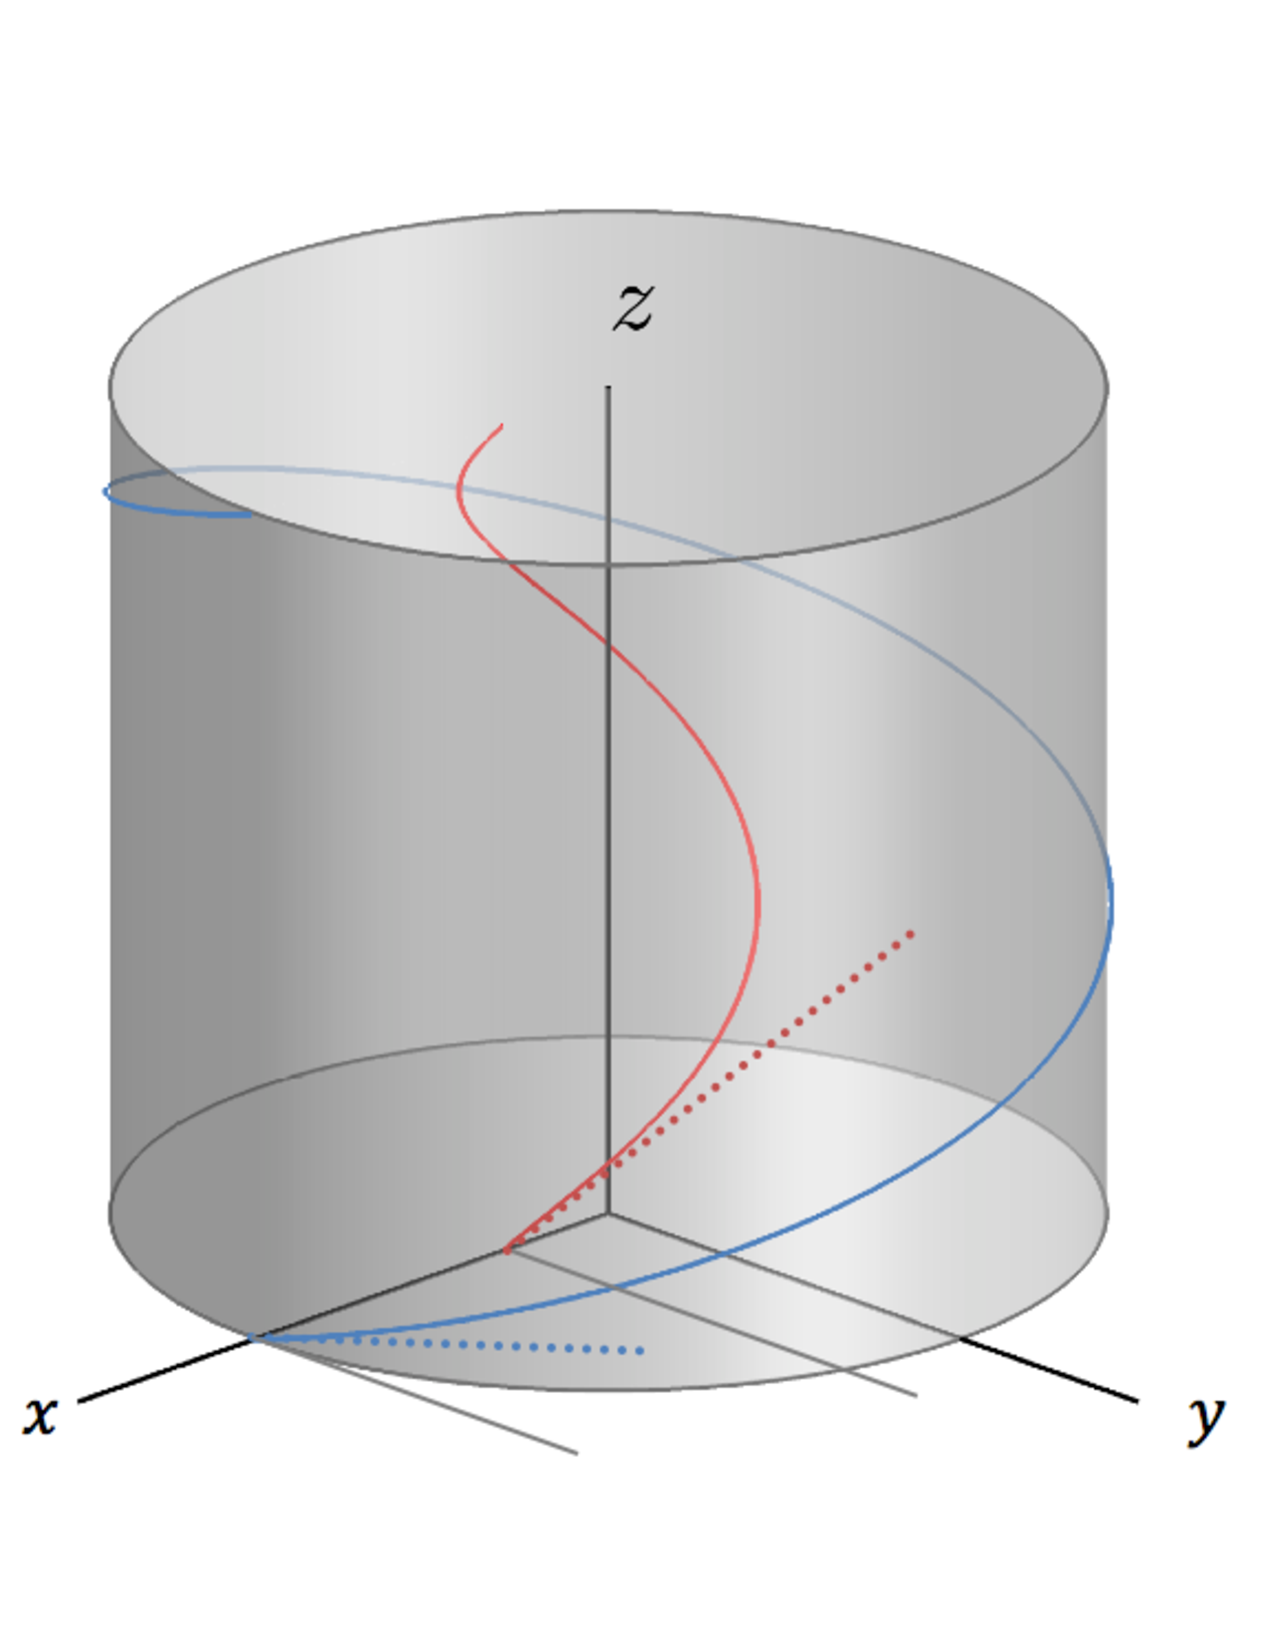
\includegraphics[width=6cm, clip = true, trim = {0in 0in  0in 0in}]{../Images/helix.pdf}
%        \caption{Twisted monofilament with lines representing polymer chain configurations after inserted twist.}
%        \label{fig:helix}
%				%%%% I like this figure but I want to adjust it - it shouldn't be r theta, it should be x & y on the horizontal axis and maybe label alpha in the picture too.  
%				
%				
%    %\end{subfigure}
%  %  \quad %add desired spacing between images, e. g. ~, \quad, \qquad, \hfill etc. 
%      %(or a blank line to force the subfigure onto a new line)
%   % \begin{subfigure}[b]{0.5\textwidth}
%    %    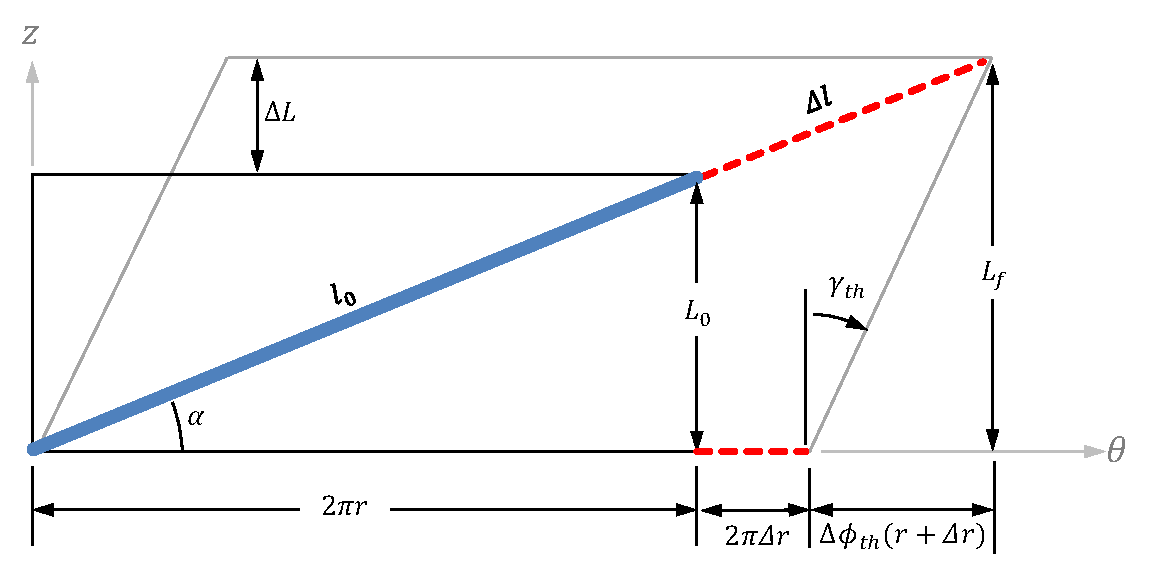
\includegraphics[width=9cm,]{../Images/1D_thermal_kinematic_v2.pdf}
%     %   \caption{}
%     %   \label{fig:1D_thermal}
%    %\end{subfigure}
%    %\caption{(\subref{fig:helix}) A section of precursor fiber after inserting twists. Polymer chains highlighted in blue showing variable angle as a function of radius. (\subref{fig:1D_thermal}) Polymer chain before and after heating with shear modulus assumed to be negligible. Dark blue line is original length of single wrap of polymer chain at some radial position. Untwist angle $\phi_{th}$ shown as negative because positive angles are taken as twists about the $z$-axis of the fiber}
%  %  \label{fig:1D_conceptual}
%\end{figure} 

%\begin{figure}
%    \centering
%   % \begin{subfigure}[b]{0.3\textwidth}
%        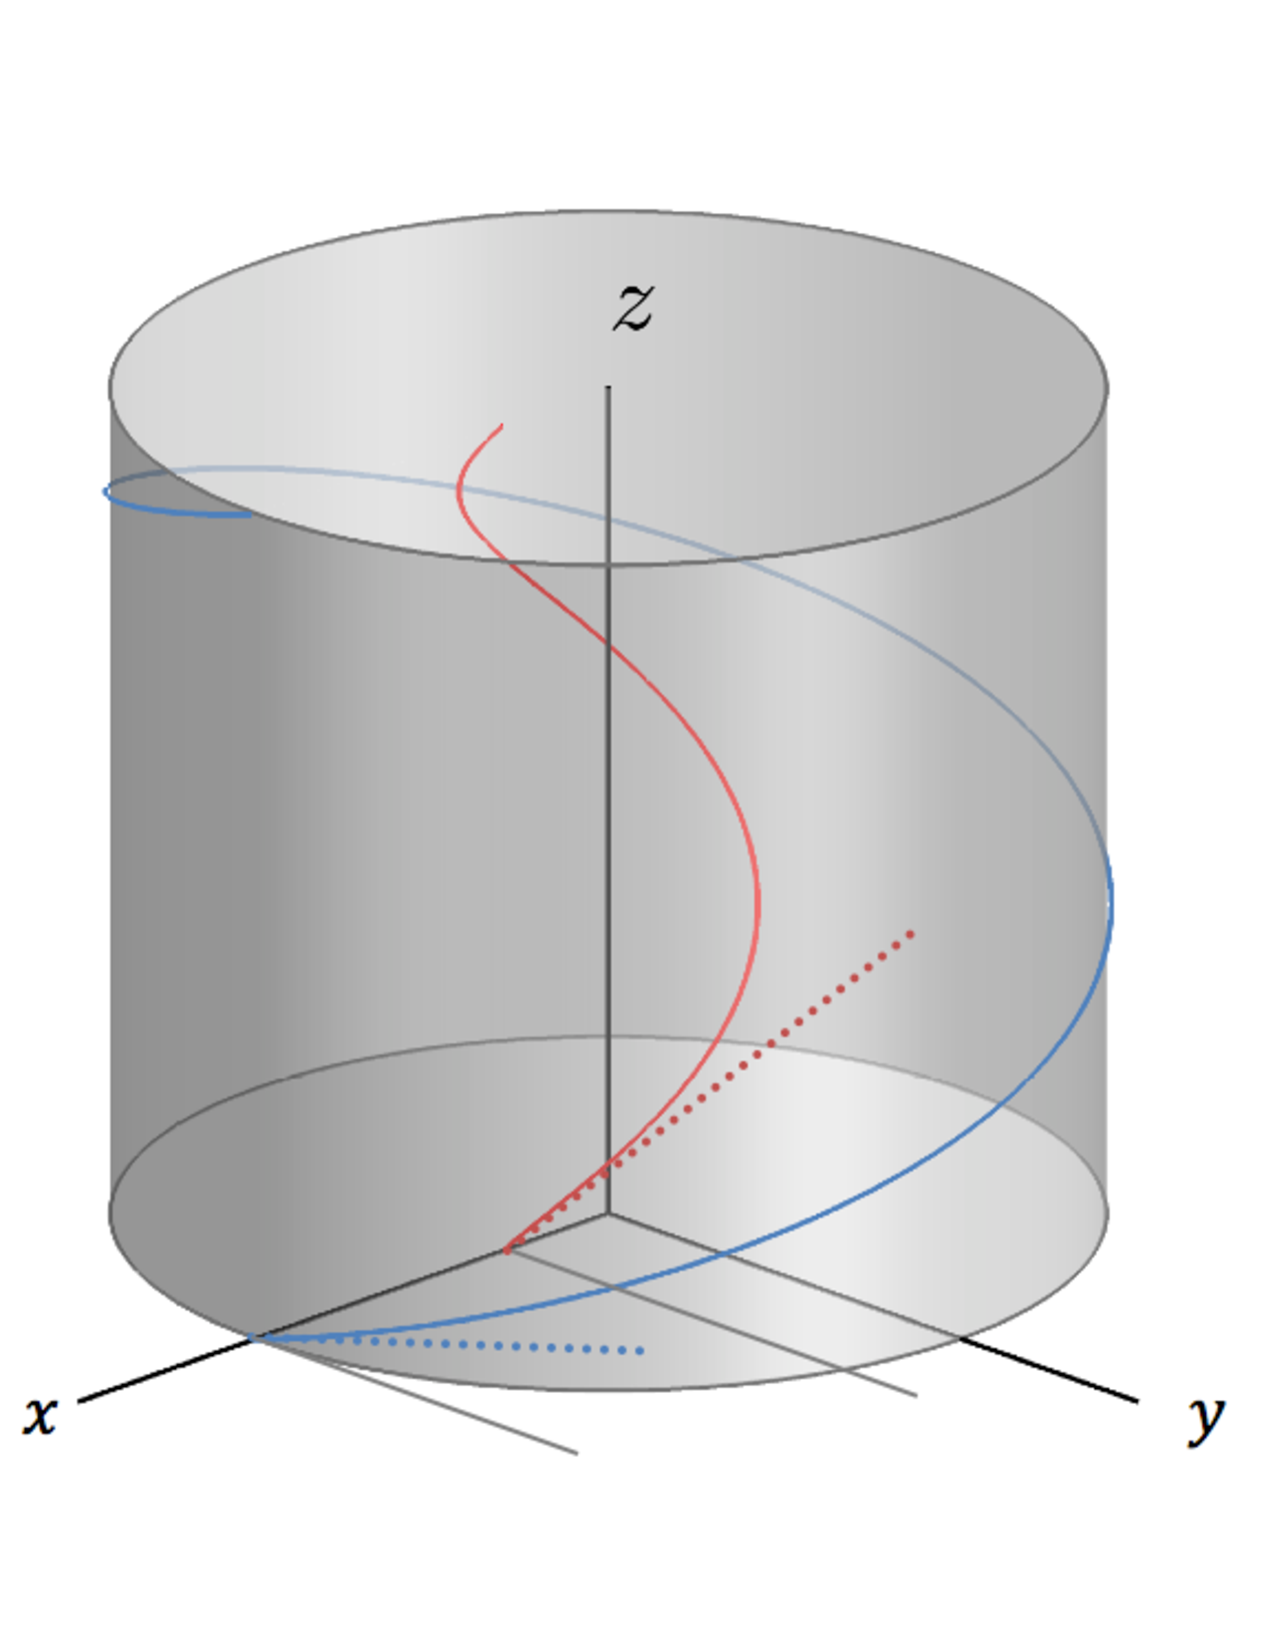
\includegraphics[width=6cm, clip = true, trim = {0in 0in  0in 0in}]{../Images/helix.pdf}
%        \caption{Twisted monofilament with lines representing polymer chain configurations after inserted twist.}
%        \label{fig:helix}
%\end{figure} 
%
%

%\begin{figure}
%    \centering
%     \begin{subfigure}[b]{0.5\textwidth}
%        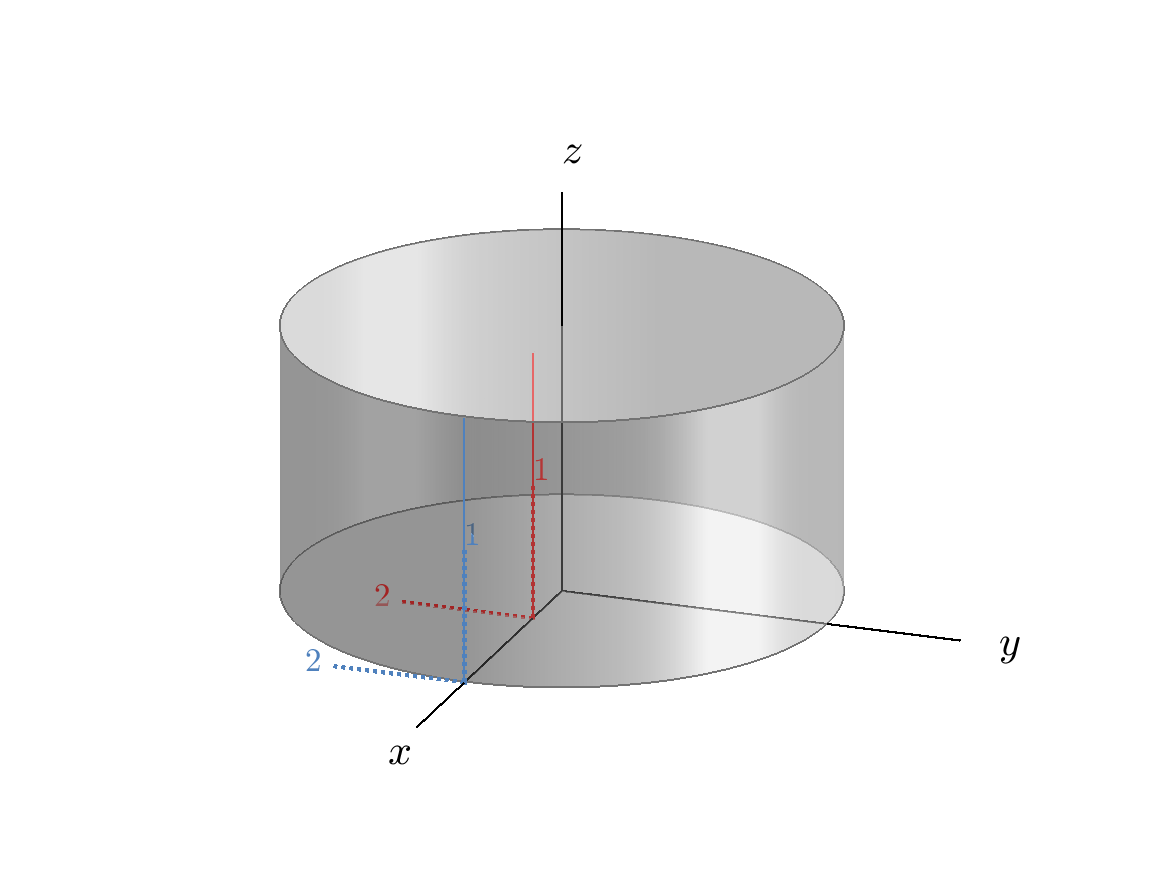
\includegraphics[width=9cm, clip = true, trim = {1in 1in  1in 1in}]{../Images/helix_2_initial.pdf}
%        \caption{Initial configuration }
%        \label{fig:helix_init}
%        \end{subfigure}
%     \begin{subfigure}[b]{0.5\textwidth}
%        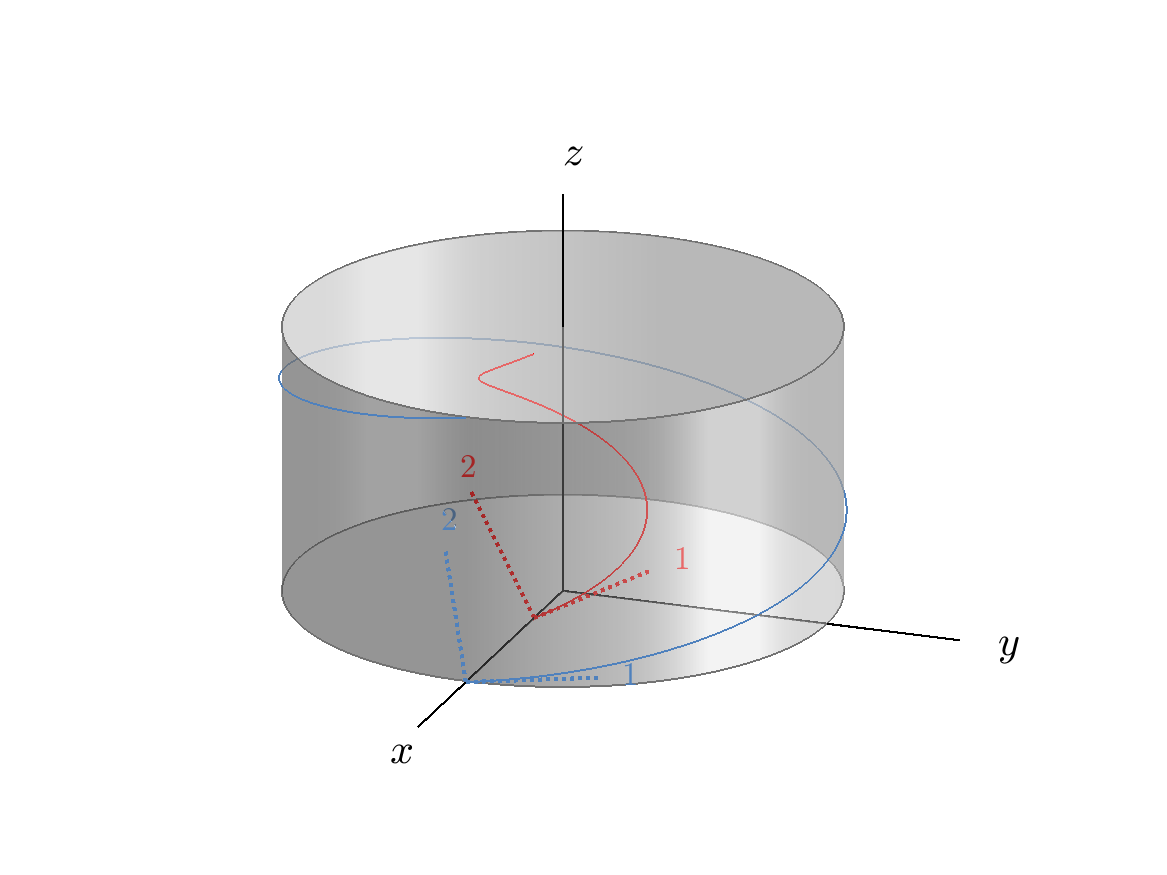
\includegraphics[width=9cm, clip = true, trim = {1in 1in  1in 1in}]{../Images/helix_2.pdf}
%        \caption{Twisted and annealed configuration}
%        \label{fig:helix_final}
%        \end{subfigure}
%        \caption{Conceptual diagram showing (\subref{fig:helix_init}) untwisted and (\subref{fig:helix_final}) twisted monofilament with lines representing polymer chain configurations. Notices that angle of polymer chain with respect to the $x-y$ place depends on radial position after twisting, but not before.}
%        \label{fig:helix}
%\end{figure}
%
\begin{figure}
    \centering
     \begin{subfigure}[b]{0.5\textwidth}
        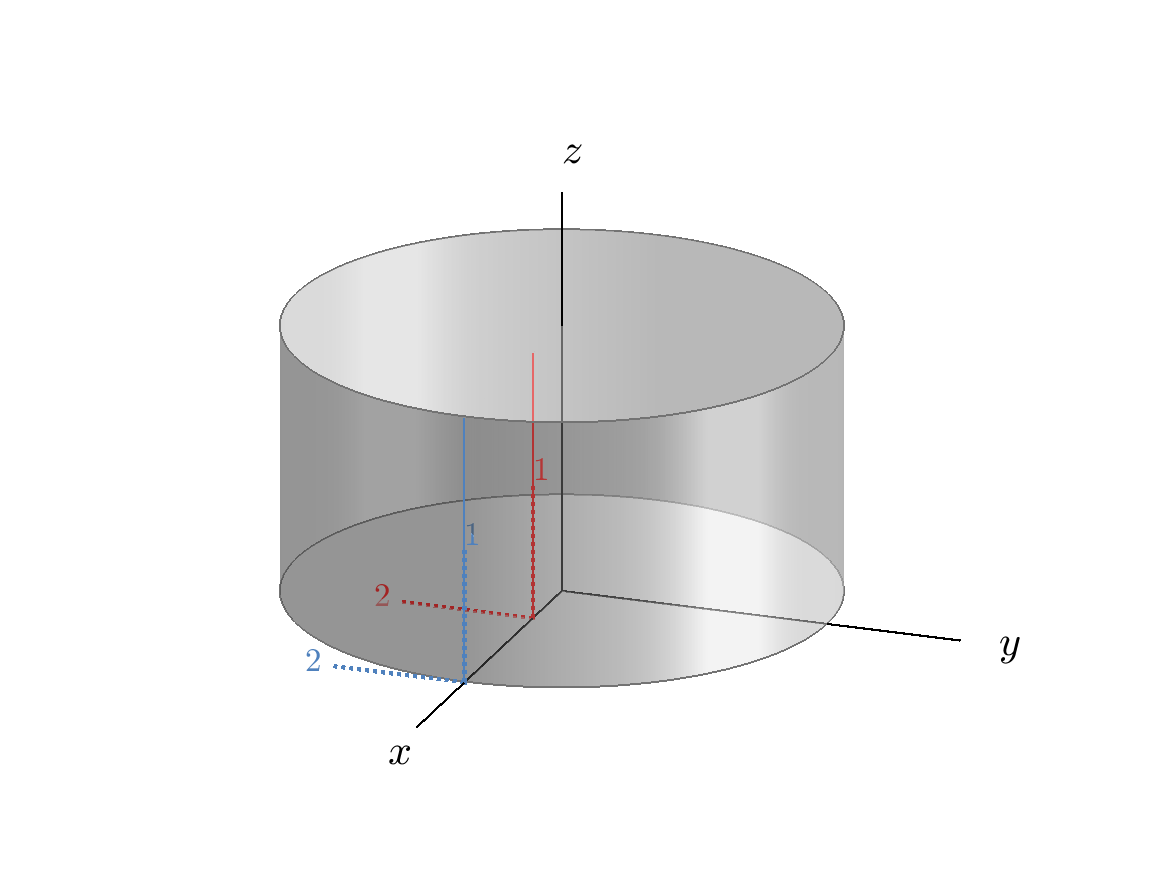
\includegraphics[width=7cm, clip = true, trim = {0.8in 0.5in  0.8in 0.8in}]{../Images/helix_2_initial.pdf}
        \caption{Initial configuration }
        \label{fig:helix_init}
        \end{subfigure}
     \begin{subfigure}[b]{0.5\textwidth}
        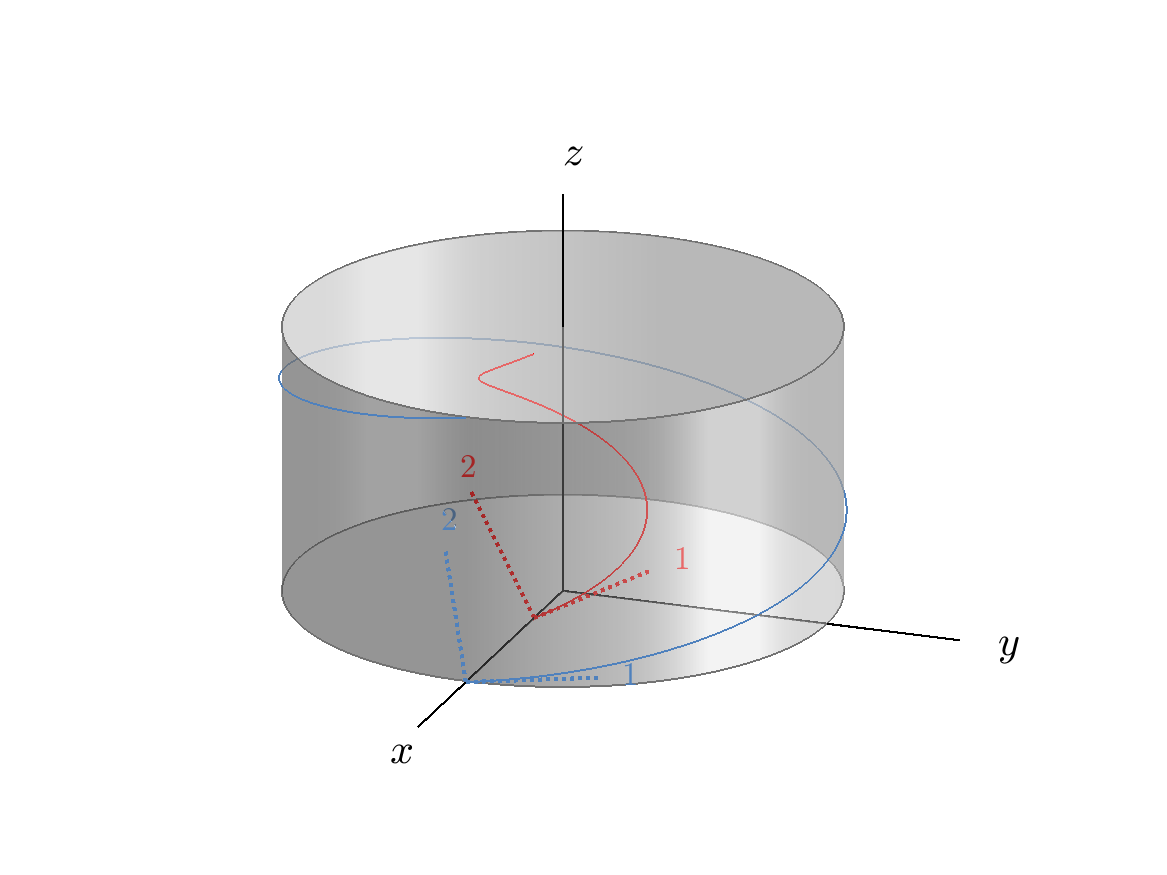
\includegraphics[width=7cm, clip = true, trim = {0.8in 0.5in  0.8in 0.8in}]{../Images/helix_2.pdf}
        \caption{Twisted and annealed configuration}
        \label{fig:helix_final}
        \end{subfigure}
        \caption{Conceptual diagram showing (\subref{fig:helix_init}) untwisted and (\subref{fig:helix_final}) twisted monofilament with lines representing polymer chain configurations. Notices that angle of polymer chain (1-direction) with respect to the $x-y$ plane ($\alpha$) depends on radial position after twisting.}
        \label{fig:helix}
\end{figure}

% \begin{figure*}
%    \centering
%   % \begin{subfigure}[b]{0.3\textwidth}
%%        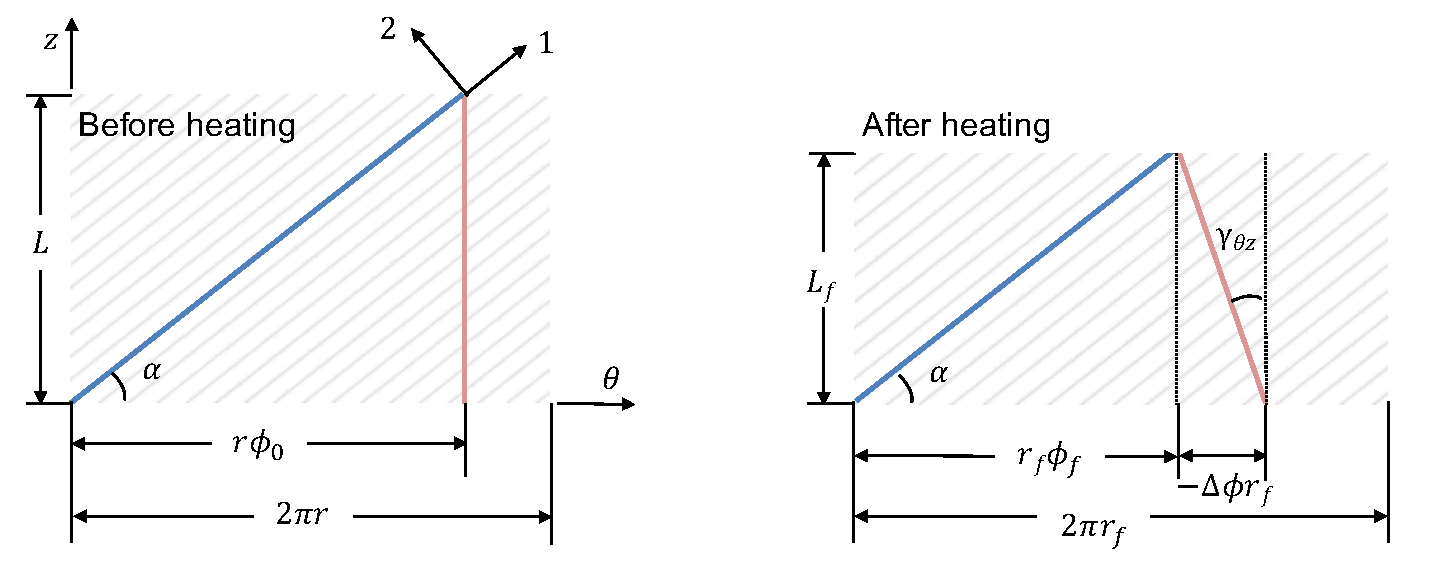
\includegraphics[width=15cm ]{../Images/unwrapped_2_both.pdf}
%        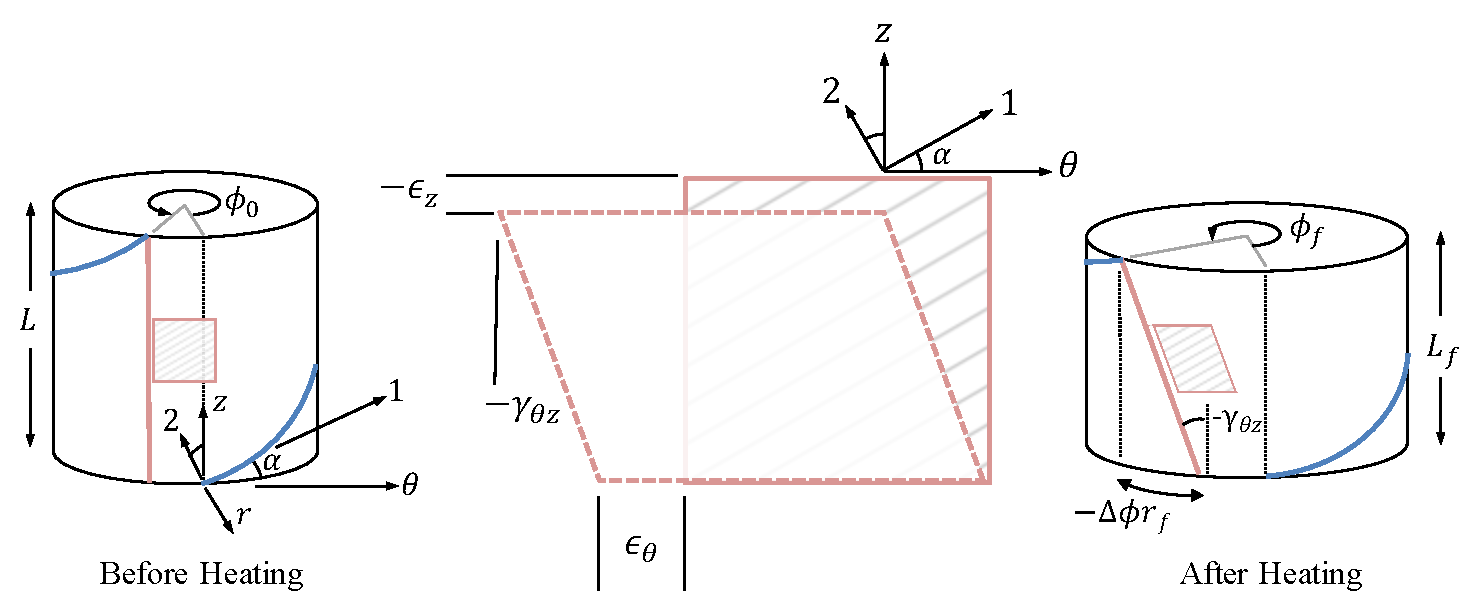
\includegraphics[width=14cm , clip = true, trim = {0in 0in  0in 0.1in}]{../Images/elemental_diagram_2}
%        \caption{Sections of TPA before and after heating with elemental 2D section shown on both, as well as enlarged between the two. The elemental section shows shear, axial, and tangential strains resulting from thermal loading of a twisted polymer. Radial ($r$), tangential ($\theta$) and axial ($z$) coordinates, as well as the polymer chain coordinates (1 \& 2 directions) are shown. Notice that 1 and 2 directions are rotated from $\theta$ and $z$ directions by angle $\alpha$.  This rotation is due to the initial twist angle shown as $\phi_0$, which is maintained due to annealing.  The initial angle $\phi_0$ is changed to $\phi_f$ after heating as a result of a thermally induced twisting by angle $-\Delta\phi$.}
%        \label{fig:unwrapped}
%\end{figure*}
%
%
%To date, research on TPAs and TCPAs has focused on experimentally exploring the actuation phenomenon and characterizing actuator performance \cite{haines_artificial, mirvakili_simple, cherubini_experimental, moretti_experimental}. Due in part to the novelty of these devices, the complex geometry of the coiling, and the experimental challenges in model validation, there is limited work on the analytic modeling of these synthetic actuators.  Because of their simpler geometry, the modeling work to date has focused on TPAs rather than TCPAs. 
%Aziz et al. \cite{aziz_controlled} used the thermal expansion properties of twisted fibers along with classical torsion theory to model TPAs and got good agreement with experimental results for both torsional stroke, i.e. untwist, and blocked torque, i.e. torque that develops when the heated fibers are securely clamped.  However, using thermal expansion of the twisted fibers for design purposes can be limiting because it requires experimental tests whenever a new initial twist is inserted.  Additionally, their work assumed no length changes in the twisted fibers. 
%
%\begin{figure}
%    \centering
%   % \begin{subfigure}[b]{0.3\textwidth}
%        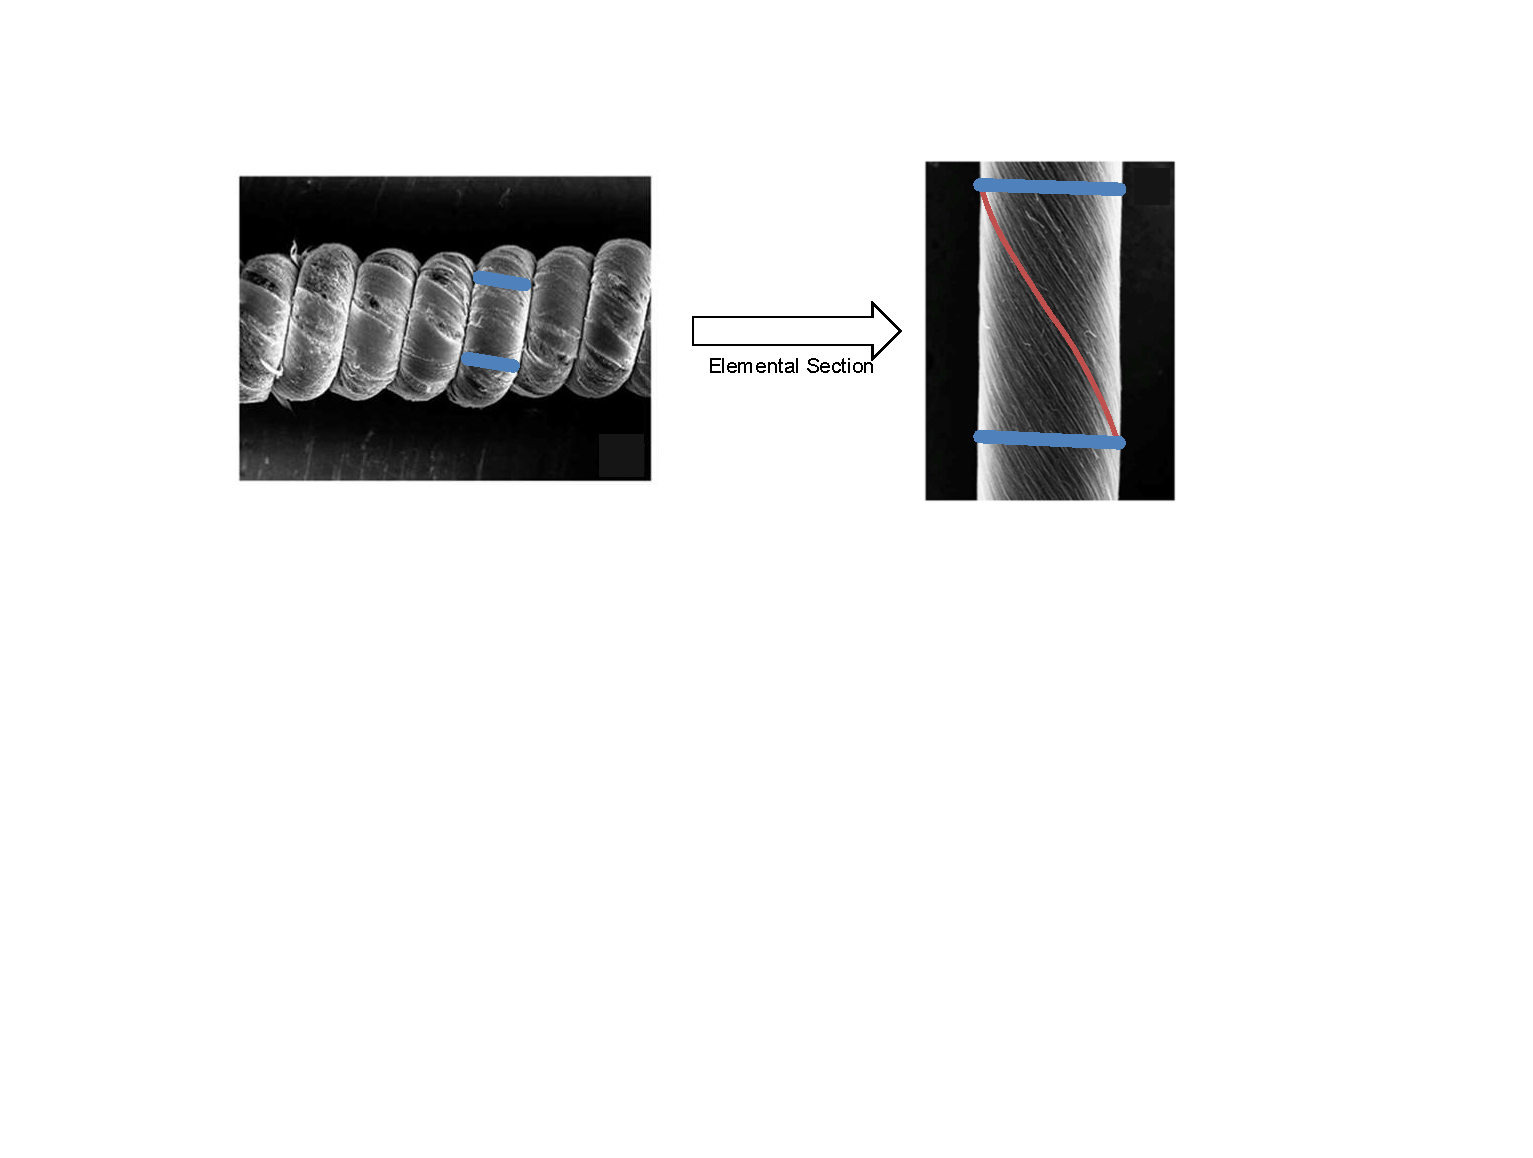
\includegraphics[width=9cm, clip = true, trim = {1in 3.5in  1in 0.5in}]{../Images/coiled.eps}
%        \caption{Twisted coiled polymer actuator (TCPA) on the left and twisted polymer actuator (TPA) on the right which can be considered an elemental section of the TCPA. Adapted from [Haines et al. 2014].}
%        \label{fig:coiled}
%\end{figure}
%


\section{Fabrication of torsional twisted polymer actuators}

\begin{figure}
    \centering
        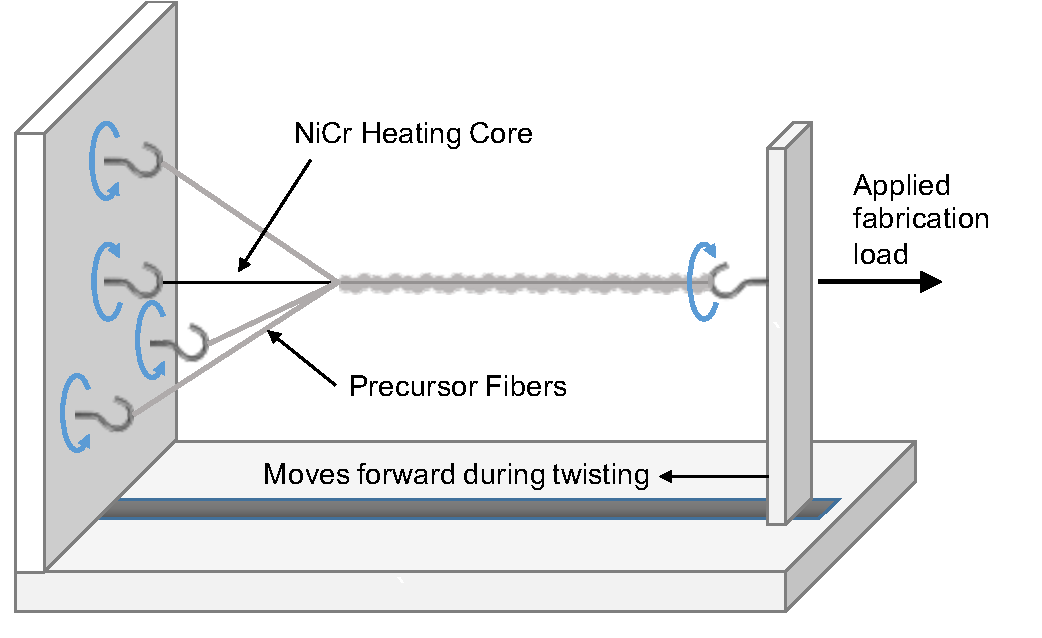
\includegraphics[width=8cm]{../Images/coiling_rig.pdf}
        \caption{Fabrication rig for torsional TPA based on twisted rope fabrication process. During the twisting process the precursor fibers are twisted in a direction opposite to that of the hook on the right. If a central heating or structural core is use, the center hook on the left is turned at the same rate as that on the right to maintain zero twist in the core. }
        \label{fig:coiled}
\end{figure}

\section{Methods for isotonic torsional stroke testing}
In order to characterize these torsional actuators, an experimental setup was designed and built which maintained a constant torque on the actuators during heating. A preload torque is known to be required to bring these actuators back to their initial angle state after cooling. The experimental setup included a 3D printed frame, ball bearing, torque spool, clamp, and weight. This setup can be see in figure \ref{fig:setup}. In this figure, the actuator sample can be seen to be clamped on the right of the frame. The left side of the sample is glued into the torque spool, a hollow pulley that interfaces with a bearing pair. A pair of ball bearings are used to react both the moment and radial loads passed into the torque spool from the weight. This weight hangs from the 6 mm diameter torque by a fine steel wire. 

The position of the weight is measured using a Polytec OVF-5000/OVF-534 vibrometer controller and sensor unit, along with DD-900 Digital Displacement Decoder unit. The voltage output of this system is linearly related to a change of position of the object on which it focuses. This voltage is recorded by a National Instruments PXI-XXXX multifunction data acquisition card, which simultaneously samples temperature measurement from the K-type thermocouple embedded within the test sample as shown in figure \ref{fig:setup}. Ambient room temperature is noted from the sample temperature prior to the application of a thermal load. Temperature and displacement measurements are recorded at 100 Hz. 

Each test is initiate by clamping an actuator sample in a frame and applying a preload torque by attaching a weight to the cable on the torque spool. The laser vibrometer zero position is then reset, and the data acquisition system is started. A hot air source is then placed adjacent to the sample to heat the actuator. When the temperature of the actuator reaches between 90-100$^\circ$C the heat source is removed, as temperatures above 120$^\circ$C are known to anneal the nylon precursor fibers. The actuator is then allowed to cool under free convection until the internal temperature returns to the pre-heating condition. Samples that return to their initial angle after this cooling period are reused in subsequent tests, but those that maintained a non-zero final displacement angle were discarded after testing. 



\begin{figure}
    \centering
        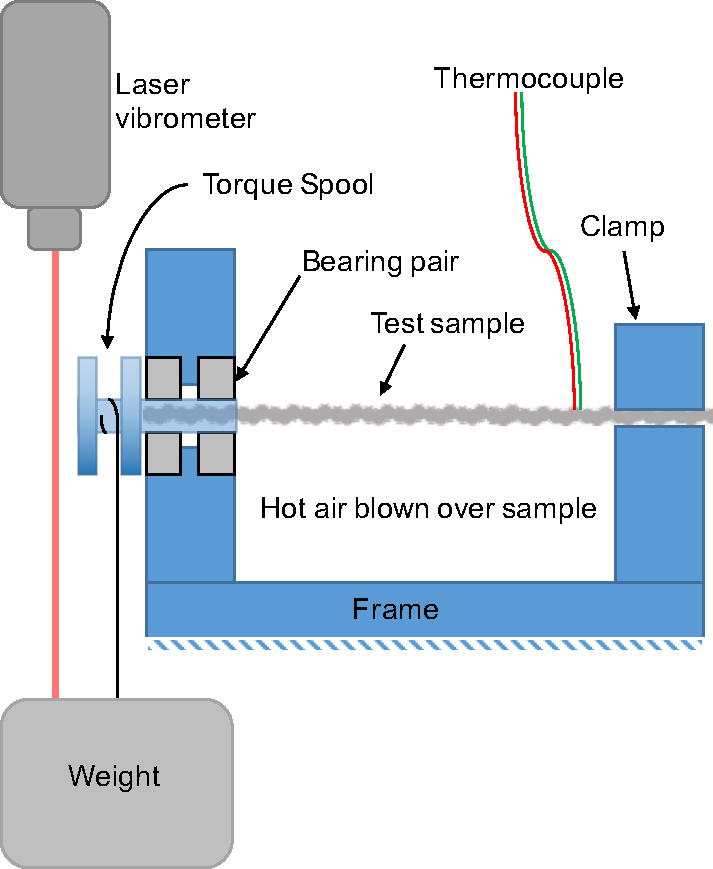
\includegraphics[width=6cm]{../Images/experimental_setup.pdf}
        \caption{Isotonic experimental testing rig for measuring actuation stroke under thermal loading.}
        \label{fig:setup}
\end{figure}

\section{Experimental Results}


\section{Discussion}

\section{Conclusions}




\bibliography{../../../LITERATURE/ALL_REFS}

\bibliographystyle{asmems4}





\end{document}

